\documentclass[10pt,a4paper]{article}

% Nastavitve strani
\setlength{\oddsidemargin}{-0. cm} %
\setlength{\evensidemargin}{-0. cm}%
\setlength{\topmargin}{-0.54 cm}   %
\setlength{\textwidth}{16. cm}     %
\setlength{\textheight}{24 cm}     %
\setlength{\marginparsep}{3 mm}    %
\setlength{\marginparwidth}{1.5 cm}%

\usepackage{parskip}
\usepackage{url}
\usepackage[slovene]{babel}
\usepackage[utf8]{inputenc}
\usepackage{graphicx}
\usepackage{subfig}
\usepackage{changepage}
\usepackage{amsmath}
\usepackage[affil-it]{authblk}
\usepackage{longtable}
\usepackage{float}
\usepackage{verbatim}



%Literatura
\bibliographystyle{unsrt}

\begin{document}
\begin{titlepage}
	\begin{center}
		\large UNIVERZA V LJUBLJANI
		\\[1cm]
		\large FAKULTETA ZA STROJNIŠTVO
		\\[5cm]
		\large Poročilo - Magistrski praktikum
		\\[0.5cm]
		\Large\textbf{Algoritem glajenja poti za avtonomno vodena vozila}
		%\\[0.5cm]
		%Sistem z vec prostostnimi stopnjami SisVPS-03
		\\[4cm]
		Martin Knap, 23172069
		\\[0.5cm]
		Mentor: doc. dr. Rok Vrabič
		%\\[0.5cm]
		%Asistent: dr. Gregor Čepon
		\\[5cm]
		Ljubljana, 30. 4. 2018
	\end{center}
\end{titlepage}

\tableofcontents
\listoffigures
\clearpage

% porocilo zahteva: 1. definicja problema, 2. namen in cilji, 3. metode raziskovanja, 4. predvidene predpostavke in omejitve, 5. literatura

\section{Uvod}

Pri razvoju avtonomnega vozila, namenjenega razvozu materiala po proizvodnih prostorih, smo se soočili s problemom pri gibanju vozila. Problem se pojavi pri ubiranju poti, ki jo tvori navigacijski algoritem vozila. Ta pot vodi vozilo tako, da se le-to giblje energijsko neučinkovito ter sunkovito. Posledice takšne, grobo tvorjene poti se odražajo v hitrejšem praznenju baterij. To pomeni, da je potrebno baterije vozila večkrat polniti, ter da je vozilo manj časa razpoložljivo. Problem predstavlja tudi potencialno nevarnost, da vozilo zaradi sunkovitih gibov izgubi svoj tovor.

Naša naloga je bila izboljšati pot, ki jo tvori navigacijski algoritem in posledično omogočiti vozilu, da bo delovalo energijsko učinkovitejše, zanesljivejše, ter da bo vozilo na razpolago daljše časovno obdobje.

\section{Ozadje problema}

Problem torej izvira iz poti, ki jo ustvari navigacijski algoritem vozila. Preden se lotimo podrobnejše obravnave izvora težav, bi bilo smotrno predstaviti zgradbo avtonomnega vozila in sistem, ki nam omogoča upravljanje z vozilom, ki se imenuje \textit{Robot Operating System} ali krajše ROS.

\subsection{Zgradba avtonomnega vozila}

Obravnavano vozilo je tipičen predstavnik robotov z diferencialnim pogonom koles (\textit{angl.: differential wheeled robot}).
Roboti te vrste imajo dve pogonski kolesi, pri čemer ima vsako od koles svoj motor. Poleg dveh pogonskih koles pa imajo ponavadi še eno ali več prosto vrtečih se koles za zagotavljanje stabilnosti. Če se pogonski kolesi vrtita z enako hitrostjo se robot giblje v ravni liniji. Zavijanje pa se doseže tako, da se eno od pogonskih koles vrti hitreje od drugega. %dodaj sliko rabotnika

%Naše vozilo ima nosilnost x kg, tako in tako moč, hitrost, maso... (dodaj specse, sliko vozila)

\subsection{Robot Operating System}

\begin{comment}
Upravljanje z vozilom nam v celoti nudi programsko okolje \textit{Robot Operating System} (ROS). To je odprtokodno okolje, ki nudi širok nabor orodij za upravlajnje z robotom, kot so na primer krmilniki za branje senzorskih informacij, krmilniki za upravlajnje z aktuatorji, fundamentalni robotski algoritmi (kartografija, navigacija, planiranje gibanja, interpretacija senzorskih podatkov, ...) in računska infrastruktura za manipulacijo s podatki tako, da je omogočena komunikacija med različnimi komponentami kompleksnega robotskega sistema. Zelo pomembno je to, da nam ROS nudi vključevanje lastnih algoritmov.

Osnovni entiteti ROS-a sta vozlišče (\textit{node}) in komunikacijska povezava (\textit{topic}). Vozlišče je program z določeno funkcijo v sistemu, komunikacijska povezava pa služi povezovanju med vozlišči in tako omogoča tok informacij. Iformacije se med vozlišči izmenjujeo v obliki sporočil (\textit{message}), ki imajo strogo določeno obliko. ROS omogoča tudi oblikovaje lastnih sporočil.
\end{comment}
%Poleg tega nam nudi še celotno računsko infrastrukturo, ki nam omogoča manipuliranje s podatki tako, da povežemo različne komponente kompleksnega robotskega sistema in vključevanje lastnih algoritmov.
%\begin{comment}
Krmiljenje obravnavanega vozila nam omogoča programsko okolje \textit{Robot Operating System} (ROS). ROS ni operacijski sistem v pravem pomenu besede, temveč je le odprtokodno ogrodje za programiranje robotov. Ideja za platformo je ta, da je delitev idej in znanja med razvijalci enostavnejša, še bolj pomembno pa je, da nam je olajšano razvijanje celotne programske infrastrukture pri razvoju robota, saj so to naredili že drugi razvijalci pred nami.

ROS je sestavljen iz krmilnikov, ki so namenjeni branju podatkov iz senzorjev in pošiljanju ukazov aktuatorjem v dobro definiranem formatu. ROS sestavlja tudi velik in rastoči nabor fundamentalnih robotskih algoritmov, ki omogočajo gradnjo zemljevidov, navigacijo po le-teh, interpretacijo podatkov iz senzorjev, planiranju gibanj, manipuliranju predmetov in še mnogo več. Poleg tega nam nudi še celotno računsko infrastrukturo, ki nam omogoča manipuliranje s podatki tako, da povežemo različne komponente kompleksnega robotskega sistema in vključevanje lastnih algoritmov. ROS je že v osnovi porazdeljen in nam omogoča delitev delovne obremenitve med več računalniki brez težav. Nudi nam tudi nabor orodij za vizualizacijo stanja robota (Gazebo, RViz), algoritmov, za odkrivanje napak in za zajemanje senzorskih podatkov. Navsezadnje pa nam širši ekosistem ROS-a nudi obsežen nabor virov, kot je spletna enciklopedija ter forum, kjer se postavljajo vprašanja ter deli znanje.

ROS torej tvori množica programov, ki delujejo istočasno in komunicirajo med sabo tako, da si med sabo pošiljajo sporočila (\textit{message}), ki imajo natančno določeno obliko. Smiselna je grafična predstavitev sistema, kjer so programi vozlišča (\textit{node}), robovi pa predstavljajo komunikacijske kanale (\textit{topic}). Za primer si poglejmo spodnjo sliko (slika \ref{fig:sl1}), kjer imamo vozlišče \verb|/turtlebot_teleop_keyboard| s katerim pretvarjamo ukaze tipkovnice v sporočila oblike \verb|geometry_msgs/Twist|, ki nosijo informacijo o temu kako naj se robot premika (linearne, kotne hitrosti). Ta sporočila se nato po povezavi \verb|/cmd_vel| posreduje do vozlišča simulacijskega okolja Gazebo z istim imenom v kateremu se nahaja testni robot.

\begin{figure}[H]
	\centering
	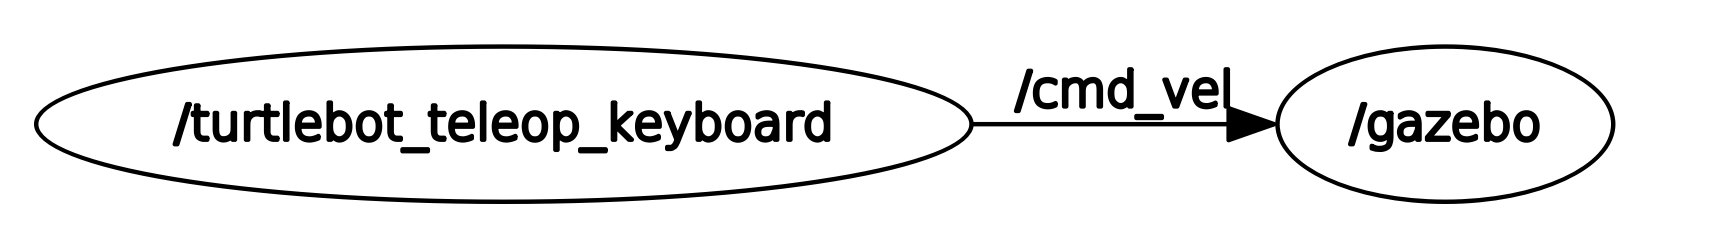
\includegraphics[width=8cm]{pic/ros.png}
	\caption{Primer dveh vozlišč z medsebojno povezavo v okolju ROS.}
	\label{fig:sl1}
\end{figure}

\subsection{Opis problema}

Seznanjeni z okvirnim delovanjem krmilnega okolja avtomatskega vozila se lahko osredotočimo na problem. Navigacija v okolju ROS se izvaja na podlagi zemljevidov uteži (angl.: \textit{costmap}). To so dvodimenzionalne mreže pravokotne oblike, kjer so ovire predstavljene z utežmi. Razdelki v zemljevidu uteži imajo tako vrednost 0 v primeru odsotnosti ovire ter vrednosti 100 v primeru ovire.

Do teh zemljevidov pridemo z uporabo kartografskih algoritmov kot je na primer \textit{Simultaneous localization and mapping} (SLAM). Mrežo okolja robota dobimo na podlagi izhodnih informacij senzorjev in sicer tako, da zaženemo kartografski algoritem in nato ročno ali avtomatsko vodimo robota po okolju tako, da zajamemo celotno okolico. Ko imamo zajeto celotno območje lahko izvozimo mrežo v obliki slike. Kartografske algoritme nam nudi okolje ROS. 

Mreže, ki jih uporabljamo v ROS-u so v obliki rastrske sivinske slike. Črna polja mreže predstavljajo mesta v prostoru kjer so ovire, kjer se robot ne more gibati. Bela polja predstavljajo mesta v prostoru kjer ni ovir in tam se robot v splošnem lahko giblje. Siva polja pa predstavljajo območje, ki ga ne poznamo.

Izvor našega problema leži v ločljivosti zemljevida uporabljenega za navigacijo. Zaradi velikih dimenzij prostorov v katerih bo robot deloval se pojavi potreba po grobih zemljevidih, saj se tako prihrani računski čas ter prostor v računalniškem spominu. Posledica uporabe zemljevida z nizko ločljivostjo, velikim korakom mreže je v majhnemu številu točk na podlagi katerih navigacijski algoritem tvori pot vozila. Pot je v temu primeru groba in izrazito robata. Na spodnji sliki vidimo z modro obarvano idelano pot, z rdečo pa je obarvna pot določena na podlagi zemljevida vrednosti pri dveh različnih ločljivostih. Z neskončno majhno diskretizacijo prostora, bi rdeča in modra pot sovpadali.

\begin{figure}[H]
	\centering
	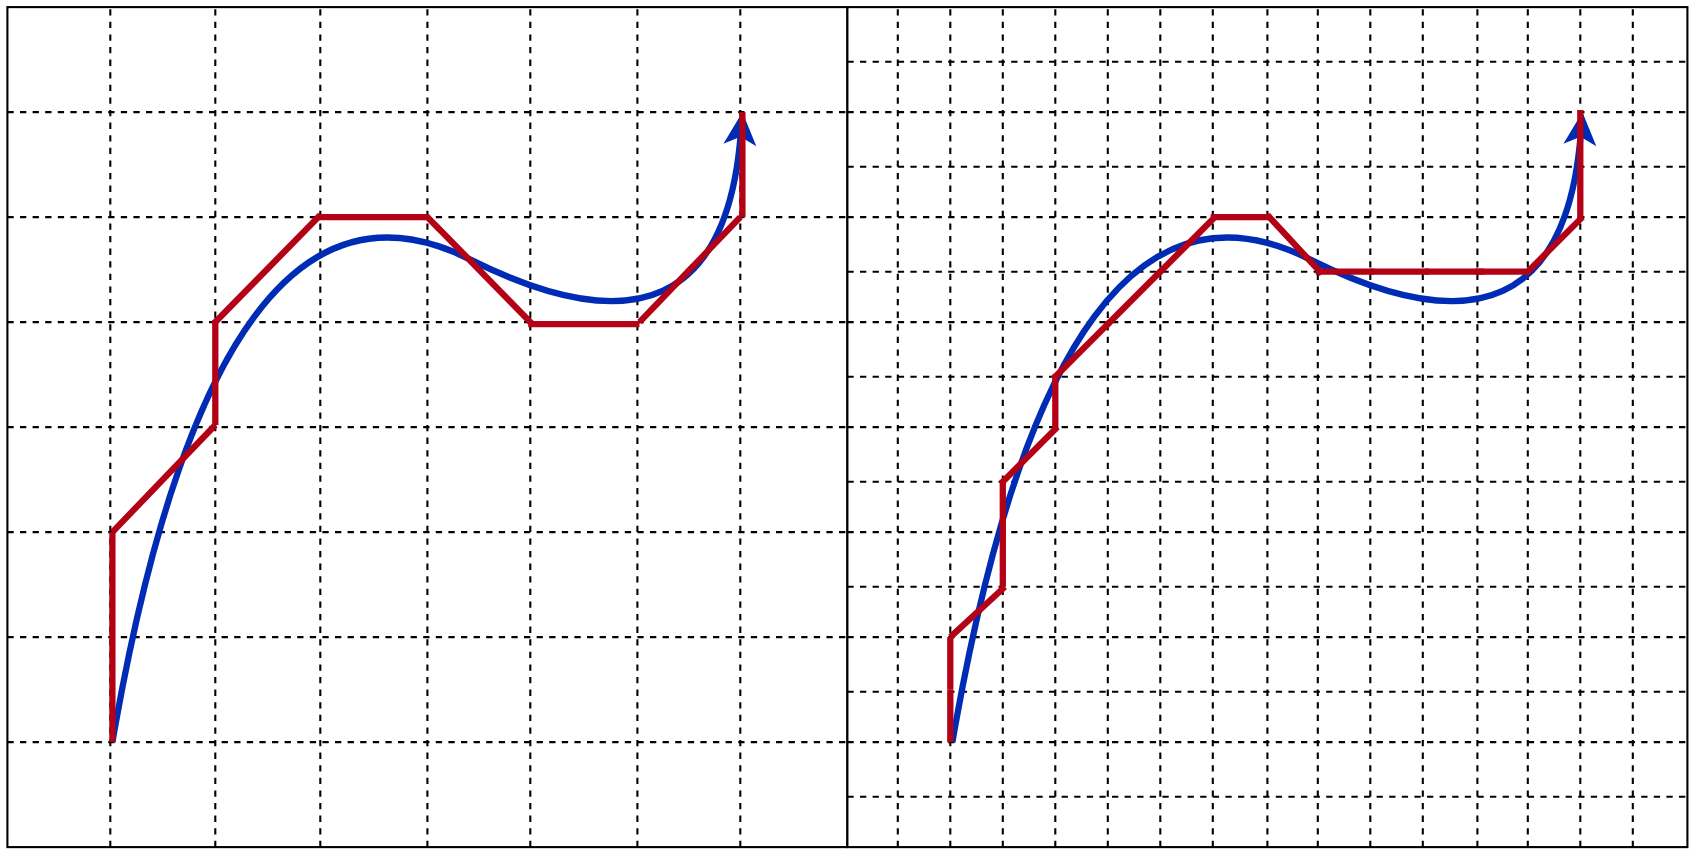
\includegraphics[width=9cm]{pic/pot.png}
	\caption{Primerjava poti, ki ju tvori navigacijski algoritem.}
	\label{fig:slika}
\end{figure}

\begin{comment}
Naša naloga je torej najti metodo, ki nam bo omogočala transformacijo nabora točk, ki tvorijo grobo pot v tak nabor točk, ki bo tvoril zglajeno, energijsko učinkovitejšo pot vozila. V kontekstu okolja ROS bo rešitev izvedena tako, da se bo ustvarilo dodatno vozlišče v katermeu se bo izvajala transformacija. To vozlišče bo bralo sporočila o poti, ki izhajajo iz ustreznega vozlišča navigacijskega algoritma, jih transformirala in pošiljala naslednjemu vozlišču, ki je izvaja sledenje poti.
\end{comment}

\section{Namen in cilji}

Kot smo spoznali v prejšnjem poglavju je uporaba zemljevidov z visko ločljivostjo neupravičena, saj je poraba računalniških sredstev tako prevelika. Naša naloga je najti način glajenja grobe poti, osnovane na zemljevidu z nizko ločljivostjo ter rešitev implementirati. V kontekstu ROS-a bo potrebno ustvariti vmesno vozlišče, ki bo prestreglo sporočila grobe poti, jih transformirala v gladko pot ter posredovla avtonomnemu vozilu. Pri implemetaciji je zaželena tudi enostavnost in intuitivnost implemetacije rešitve skozi oči uporabnika.

\section{Pregled možnih rešitev}

Navdih za rešitev problema glajenja poti smo dobili na področju motornih športov. Tam se vozniki dirkalnih vozil izključno poslužujejo načina vožnje skozi ovinke, ki se mu pravi dirkalna linija (\textit{angl.: racing line}). Dirkalna linija je pot preko ovinka, ki vozniku dirkalnika omogoča najkrajši čas proge. Želja je, da je hitrost pri vožnji skozi ovinek karseda konstantna.

\begin{figure}[H]
	\centering
	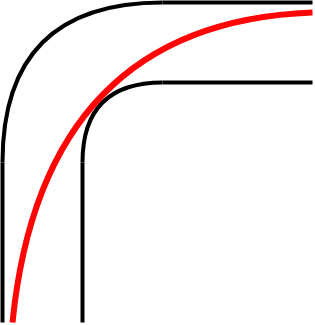
\includegraphics[width=3cm]{pic/slika4.png}
	\caption{Dirkalna linija.}
	\label{fig:slika}
\end{figure}

Ideja za dirkalno linijo je ta, da se vozilo oklepa zunanjega roba ovinka pri vstopu v ovinek in se skuša karseda približati notranjemu robu ovinka na njegovem vrhu. Na izhodu iz ovinka pa se vozilo ponovno približa zunanjemu robu. V teoriji je optimalna pot skozi ovinek takšna, ki ima največji radij.

Iskanje najboljše dirkalne linije za dano vozilo, na dani progi je eden od večjih problemov s katerim se srečujejo razvijalci dirkalnih računalniških iger. Komercialne dirkalne igre se ponavadi zanašajo na dirkalne linije, ki jih zasnujejo ljudje - strokovnjaki s področja dirkanja. Obstajajo pa tudi izjeme, ki se izognejo omenjeni metodi in se problema lotijo na povsem drugačen način. Dober primer je Colin McRae Rally, kjer dirkalno linijo računajo s pomočjo nevronske mreže, ki so jo učili strokovnjaki iz področja motornih športov. V Microsoft-ovi igri Forza Motorsport 2 s pomočjo tehnik nadzorovanega učenja (\textit{angl.: supervised learning}) učijo AI-je ter z aplikacijo evolucijskega računanja (\textit{angl.: evolutionary computation}) optimirajo njihove dirkalne linije.

Odprtokodne dirkalne igre se ponavadi zanašajo na hevristične pristope, ki tipično združujejo dobro prakso s hevristiko pri generaciji dirkalnih linij. Najuspešnejši primeri takšnih pristopov vključujejo K1999 algoritem, ki ga je razvil Remi Coulom in deluje na podlagi gradientnega spusta (\textit{angl.: gradient descent}) ter Simplix, ki ga je razvil Wolf-Dieter Beelitz za The Open Car Racing Simulator in bazira na preprosti hevristiki. Ostala uspešna primera sta tudi \textit{the bot}, ki ga je razvil Jussi Pajala za Robot Auto Racing Simulator (RARS) in je zasnovan na A* algoritmu ter the \textit{DougE1 bot} za RARS, ki ga je razvil Doug Elenveld, ta pa izkorišča genetski algoritem. Kljub temu, da omenjene rešitve temeljijo na različnih tehnikah je vsem skupno to, da skušajo zmanjšati ukrivlejnost poti vozila skozi ovinek, saj z manjšo ukrivlejnostjo poti vozilo lahko doseže večjo hitrost brez zdrsa.

Zgoraj omenjene metode so sicer zelo impresivne, vendar obstajajo tudi metode, ki upoštevajo dinamski model vozila pri reševanju omenjenega problema in vodijo do še ustreznejših rešitev omenjenega problema. Na drugi strani pa imamo rešitve, ki so malce preprostejše kot je uporaba kubičnih parametričnih Bézier krivulj pri generaciji dirkalne linije in pa edinstvena rešitev, ki jo nudi odprtokodni Vamos Avtomotive Simulator, kjer je za doesganje manjše ukrivlejnosti poti skozi ovinek uporabljena vergia masnih točk, ki jih povezuje torzijska vzmet. Do zglajene poti pridemo tako, da najdemo minimum potencialne energije shranjene v vzmeteh. Pri reševanju našega problema smo se odločili za seldnjo metodo, zato jo bomo v naslednjem poglavju predstavili podrobneje.

%\section{Algoritem glajenja poti - Vamos}
\section{Izbrana rešitev}

Vamos Avtomotive Simulator (VAS) je odprtokodno simulacijsko okolje s poudarkom na fizičnemu modeliranju \cite{VAS}. Vamos modelira veliko večino ključnih podsistemov avtomobilov, kot so elementi pogonskega sklopa in sicer motor, sklopka, menjalnik in diferencial z omejenim zdrsom. Prav tako pa je modelirano tudi obnašanje pnevmatik pri temperaturnih vplivih, vzmetenje avtomobila in aerodinamski učinki na avtomobilih. VAS igralcem nudi tudi igranje proti računalniškemu nasprotniku. V ta namen so razvijalci ustvarili algoritem izgradnje poti za računalniškega nasprotnika tako, da igralcem nudijo karseda realističen izziv. Ta algoritem bomo v naslednjem delu besedila vzeli pod drobnogled in ga nato tudi uporabili pri reševanju našega problema.

Pot vozila na začetku predstavlja nabor točk, ki tvorijo središčnico znotraj proge. Točke predstavimo kot masne točke, ki so med seboj povezane s torzijskimi vzmetmi.

\begin{figure}[H]
	\centering
	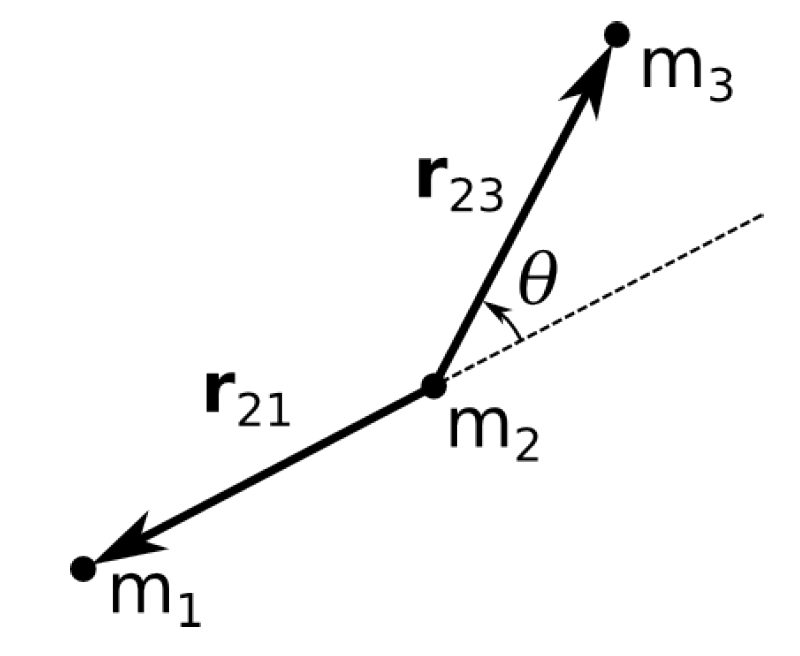
\includegraphics[width=4cm]{pic/slika5.png}
	\caption{Tri vozlišča poti. Kot $\theta$ povzorča moment \cite{VAS}.}
	\label{fig:slika}
\end{figure}

Tak sistem bo s časom silil v stanje minimalne energije v torzijskih vzmeteh in nam posledično ustvaril pot z manjšo ukrivljenostjo.

Silo, ki deluje na maso $m_2$ je možno izračunati na podlagi relativnih leg sosednjih mas. Začnimo s sklepom, da s povečanjem kota $\theta$ dobimo moment sorazmeren kotu.
\begin{equation}
\mathbf{N_2} = \mathbf{r}_{23} \times \mathbf{F_3} = -k \theta \hat{n}
\end{equation}
Pri tem je $\mathbf{r}_{23}$ vektor od $m_2$ do $m_3$ in $\hat{n}$ je enotski vektor, ki kaže v smeri $\mathbf{r}_{23} \times \mathbf{r}_{21}$. Sila na $m_3$ je tako:
\begin{equation}
\mathbf{F_3} = -\frac{k}{|\mathbf{r}_{23}|}\theta(\hat{n} \times \mathbf{r}_{23})
\end{equation}
Produkt $\theta \hat{n}$ se izračuna kot vektorski produkt $\mathbf{r}_{23}$ in $\mathbf{r}_{21}$.
\begin{equation}
\mathbf{r}_{23} \times \mathbf{r}_{21} = |\mathbf{r}_{23}||\mathbf{r}_{21}| \sin(\phi - \theta) \hat{n}
\end{equation}
\begin{equation}
\sin\theta\hat{n} = |\mathbf{r}_{23}||\mathbf{r}_{21}|\sin\theta\hat{n}
\end{equation}
\begin{equation}
\sin\theta\hat{n} = \frac{\mathbf{r}_{23} \times \mathbf{r}_{21}}{|\mathbf{r}_{23}||\mathbf{r}_{21}|}
\end{equation}
\begin{equation} \label{eq:1}
\sin\theta\hat{n} = \hat{r}_{23} \times \hat{r}_{21}
\end{equation}
Ker pričakujemo majhne kote med vozlišči lahko $\sin\theta$ zapišemo kot $\theta$.
\begin{equation} \label{eq:2}
\theta\hat{n} = \hat{r}_{23} \times \hat{r}_{21}
\end{equation}
Z vstavljanjem v enačbo $(2)$ dobimo:
\begin{equation}
\mathbf{F}_3 = \frac{k}{|\mathbf{r}_{23}|}(\hat{r}_{23} \times \hat{r}_{21}) \times \hat{r}_{23}
\end{equation}
Upoštevajoč simetrijo ugotovimo, da je $\mathbf{F}_1 = \mathbf{F}_3$ in $\mathbf{F}_2 = -2\mathbf{F}_3$ pri majhnem kotu. Definiramo lahko vektor urkivljenosti $\mathbf{c}$ pri $m_3$:
\begin{equation}
\mathbf{c} = \hat{n}/R = \theta \hat{n} / |\mathbf{r}_{23}|
\end{equation}
Kjer je $R$ radij ukrivljenosti. Kot $\theta$ je kot med $m_2$ in $m_3$ od centra ukrivljenosti.

Enačbo lahko zapišemo kot:
\begin{equation}
\mathbf{F}_3 = -k \mathbf{c} \times \hat{r}_{23}
\end{equation}
Velikost vekotrja ukrivljenosti bomo uporabili kot največjo hitrost vozila v dani točki na stezi.

Sile so izračunane za vsak povezan trojček n točk. Pri tem omejimo gibanje točk v vse smeri in namesto tega dovolimo le pomik prečno na pot. Ta omejitev nam omogoča večjo stabilnost, posledično pa lahko uporabljamo večje togostne koeficiente vzmeti in tako dobimo hitrejšo konvergenco.

Ko je izračunana skupna sila na vsakemu vozlišču lahko izračunamo novo lego točke z uporabo Newtonov-ovih zakonov gibanja ter z Euler-jevo metodo.

\begin{equation}
F = m \ddot{x} + c \dot{x}
\end{equation}

\begin{equation}
\ddot{x} = \frac{F}{m} - \frac{c}{m} \dot{x}
\end{equation}

Kvocient koeficienta dušenja in mase označimo z $d = c / m$.

\begin{equation}
\frac{\dot{x}_{i+1} - \dot{x}_i}{\Delta t} = \frac{F}{m} - d \dot{x}_i
\end{equation}

\begin{equation}
\dot{x}_{i+1} = \dot{x}_i + (\frac{F}{m} - d \dot{x}_i)\Delta t
\end{equation}

Iz definicije hitrosti sledi še druga enačba.

\begin{equation}
\dot{x} = \frac{x_{i+1} - x_i}{\Delta t}
\end{equation}

\begin{equation}
x_{i + 1} = x_{i} + \dot{x}_{i + 1} \Delta t 
\end{equation}

\begin{comment}
Z iteriranjem algoritma se lega zglajenega nabora točk stabilizira. Pri tem se je potrebno zavedati, da je pot lahko groba v ostrih ovinkih.
\end{comment}

Tako dobimo enačbo s katero lahko iterativno določimo novo lego vsake točke poti, ki jo gladimo. Algoritem vsebuje dva paramtera in sicer maso $m$ in kvocient $d$. Pri tem se je potrebno zavedati, da je nova pot lahko groba v ostrih ovinkih (glej enačbo \ref{eq:1} in \ref{eq:2}).

Spodnje slike prikazujejo delovanje dejanskega algoritma glajenja. Leva slika prikazuje graf niza točk nad katerimi bomo  izvajali glajenje. Sredinska slika prikazuje pravokotne poti po katerih bodo točke spreminjale svoj položaj z iteriranjem algoritma. Te pravokotne poti posameznih točk tvorijo tudi progo. Proga je ključna za glajenje poti, saj določa območje v katerem ga izvajamo. Na desni sliki vidimo niz točk v novi legi.

\begin{figure}[H]
	\centering
	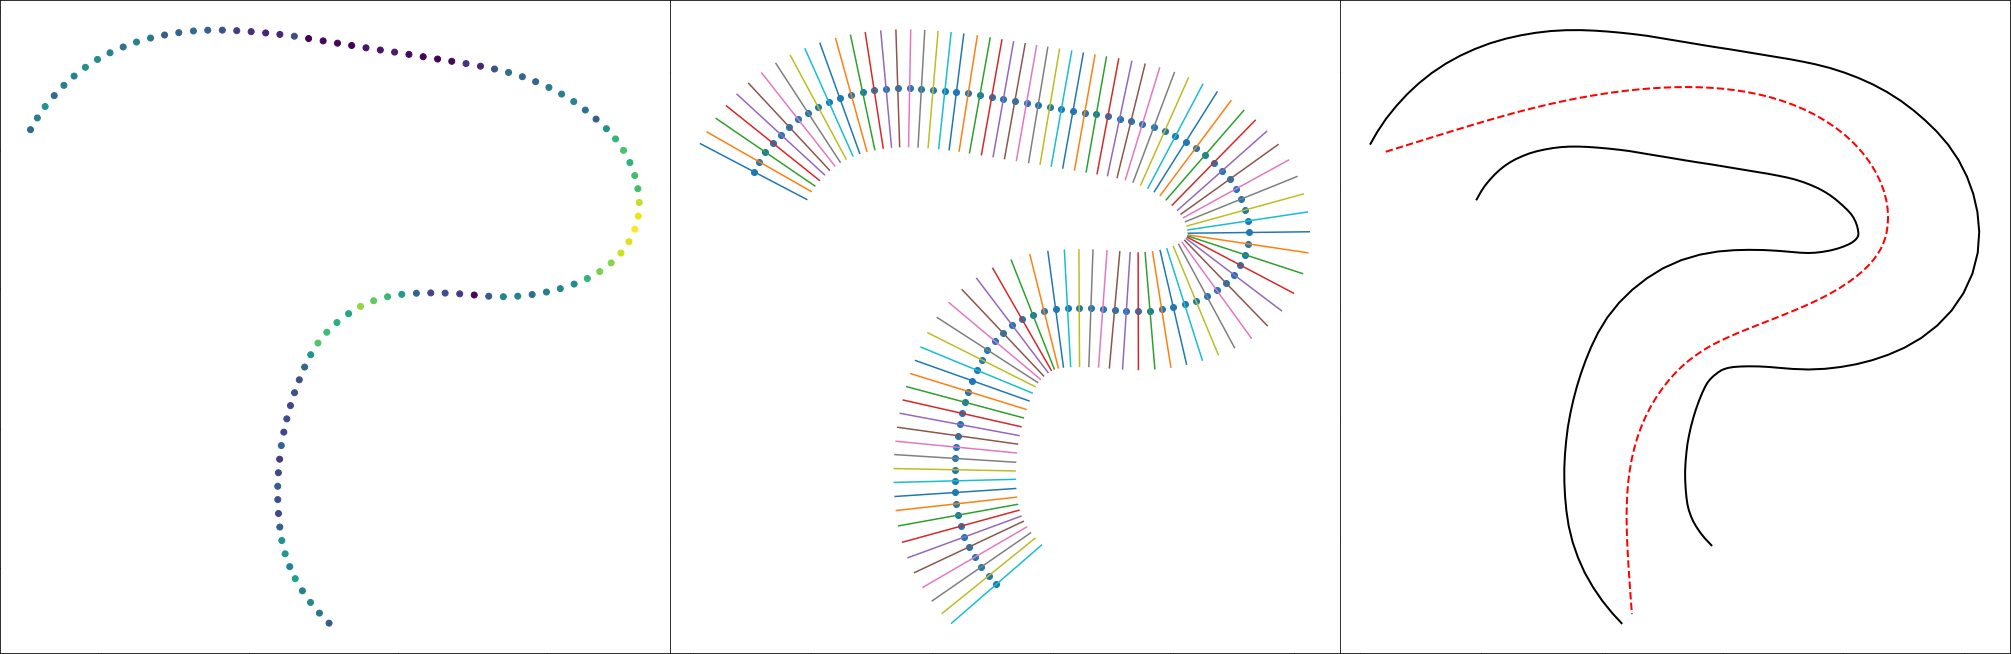
\includegraphics[width=15cm]{pic/slika6.png}
	\caption{Postopek glajenja.}
	\label{fig:slika}
\end{figure}

\section{Aplikacija algoritma}

Z znanim algoritmom glajenja sedaj lahko začnemo z reševanjem problema. Naloga je torej ustvariti vmesno vozlišče v ROS-u, ki jemlje podatke o obstoječi poti iz navigacijskega algoritma ter jih ustrezno transformira ter pošilja naslednjemu vozlišču, odgovornemu za izvajanje sledenja novo ustvarjeni poti. Pri določanju območja glajenja se bo upoštevala tudi prisotnost ovir, zato bo potrebno brati tudi informacije o zemljevidu vrednosti (\textit{costmap}). Preden zančenmo na delu s samim vozliščem pa je potrebno ustvariti okolje kjer naš program lahko preizkusimo.

\subsection{Priprava razvijalnega okolja}

Omenjeno vozilo v razvoju ni bilo lahko razpoložljivo, zato nam na srečo ROS paket nudi povezljivost s simulacijskim okoljem Gazebo. Gazebo je odprtokodno simulacijsko okolje za testiranje robotov, ki nudi dinamske simulacije, 3D prikaz, generacijo poljubnega modela robota in okolja in še marsikaj drugega. Omenjeni program smo uporabljali v kombinaciji z ROS paketom RViz, ki nudi 3D prikaz robota, okolja ter prikaz vseh vrst senzorksih podatkov, kot so na primer točke zajete z laserskim merilnikom razdalje. Še pomembnejše pa je to, da nam RViz prikazuje podatke o poti, ki jo nudi navigacijski algoritem in tako nudi takojšnjo preverbo. Da okolje izpopolnimo, potrebujemo še testno vozilo. Uporabili bomo paket, ki ga nudi spletni blog moorerobots \cite{moorerobots}, ta pa vsebuje preprosto vozilo z diferencialnim pogonom. Delali bomo z ROS izvedbo Kinetic Kame na operacijskem sistemu Linux Ubuntu. Z definiranim okoljem sedaj lahko začnemo na razvoju omenjenega vozlišča vokolju ROS.

\subsection{Izdelava vozlišča}

Za navigacijo robota v okolju ROS skrbi t.i. navigacijski sklad, katerega ključno vozlišče se imenuje \verb|/move_base|. To vozlišče na podlagi podane ciljne točke, zemljevida okolice in bližnje okolice zaznane z laserskim merilnikom ustvari globalen načrt oziroma pot ter lokalno pot, katere namen je, da skuša vozilo karseda približati globalni. Glajena bo pot globalnega načrta, ki jo \verb|/move_base| pošilja po komunikacijski povezavi (\textit{topic}) \verb|/move_base/TrajectoryPlannerROS/global_plan|. Sporočila te povezave so tipa \verb|nav_msgs/Path| in nosijo informacijo o legah točk poti ter o orientaciji v ciljni točki. Ker se pri določanju območja glajenja upošteva tudi prisotnost ovir oziroma zemljevid vrednosti je potrebno brati tudi sporočila tipa \verb|nav_msgs/OccupancyGrid|, ki jih navigacijski sklad pošilja po povezavi \verb|/move_base/global_costmap/costmap|.

Algoritem je napisan v programskem jeziku Python in je v grobem sestavljen iz petih funkcij. Naloga prve funkcije je branje obstoječe, grobe poti in tvorjenje izhodnega podatka v obliki 2D niza točk, kjer prvi stolpec predstavlja x koordinate, drugi stolpec pa y koordinate nezglajene poti. Naloga druge funkcije je dodajanje vmesnih točk med točke nezglajene poti, saj je groba pot sestavljena iz malega števila točk. Tako omogočimo, da se postopek glajenja izvaja nad večjim številom točk, kar še dodatno pripomore k tvorbi ustreznejše poti. Tretja funkcija bere zemljevid vrednosti in informacijo o zemljevidu pretvarja v matriko čitljive oblike, kjer lega posameznega elementa sovpada s točko kartografiranega prostora. V tretji funkciji se določa širina območja glajenja in sicer tako, da se inkrementalno povečuje leva in desna meja območja nakar se za vsak inkrement širine preveri, če katera od koordinat leve in desne meje leži v območju ovire. To se izvede tako, da se koordinate leve in desne meje območja glajenja prevede v pripadajoče elemente matrike vrednosti in preveri, če je pripadajoča vrednost pod mejo. Ko z inkrementiranjem dosežemo oviro je prag sprejemljive vrednosti presežen in inkrementiranje se zaključi, s tem pa določimo širino območja glajenja. Širina območja inkrementalnega povečevanja širine je omejeno, saj bi se v okolici brez ovir inkrementiranje izvajalo, do roba zemljevida. Postopek se izvajala ločeno za levo in desno mejo.

Četrta funkcija predstavlja jedro programa kjer se nahaja Vamos gladilni algoritem. V tem delu programa se torej izvaja transformacija točk prebranih iz druge funkcije. Ta funkcija vsebuje tudi vplivne parametre glajenja kot so masa točke, togostni koeficient, število iteracij algoritma ter širina proge, ki se jo določi v tretji funkciji. Izhodni podatek je ponovno 2D niz točk, le da so te transformirane. V tretji funkciji se izvaja prepis zglajenega niza točk v sporočila oblike \verb|nav_msgs/Path| ter njihovo oglaševanje po komunikacijskem kanalu \verb|/vamos|. Na ta kanal se nato poveže vozlišče odgovorno za vodenje robota po globalni poti.
\begin{comment}
\begin{figure}[H]
	\centering
	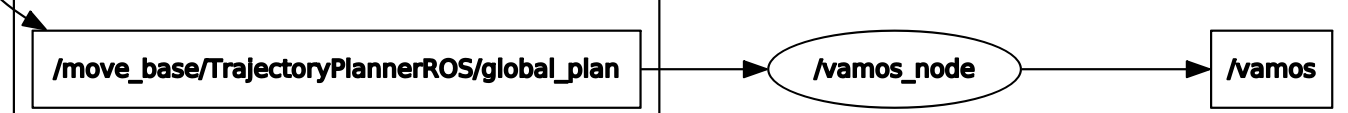
\includegraphics[width=8.9cm]{slika7.png}
	\caption{Grafičen prikaz povezav.}
	\label{fig:slika}
\end{figure}
\end{comment}
Vozlišče med drugim koristi tudi ROS-ov paket Dynamic Reconfigure, ki omogoča spreminjanje parametrov vozlišča tekom njegovega obratovanja. Z omenjenim paketom nudimo manipulacijo nad parametri v drugi, treji in četrti funkciji.




\end{document}